\documentclass{article}

\usepackage[utf8x]{inputenc}
\usepackage[spanish]{babel}
\usepackage[margin=3cm]{geometry}
\usepackage{amsmath}
\usepackage{amssymb}

\usepackage{graphicx}


\title{Computación Concurrente \\ \Large{Tarea 3}}
\author{
  Diego Goméz Montesinos
  \and
  José Emiliano Cabrera Blancas
  }
\date{25 febrero 2014}
\begin{document}
\maketitle
\begin{enumerate}
\item{
    Recuerden el modelo visto en clase con el que resolvimos la tarea
    $\epsilon$-aggremment para dos procesos. Alice y Bob proponen un valor y
    quieren quedar de acuerdo en un valor que no diste más de $\epsilon$ de lo
    que el otro decidió. Después vimos que necesitaban comunicarse y que para 
    $\epsilon$ más pequeñas se necesitaban mñas y más rondas de comunicación.
    Recuerden que usamos el modelo de memoria compartida de lectura/escrita por
    capas \textit{full information} (por cada escritura leiamos un nuevo
    arreglo y escribimos todo lo que sabemos cada vez).\\
    Ahora proponemos otros dos modelos de comunicación: el modelo chismoso y el
    modelo discusión civil. El modelo chismoso dice que si Alice y Bob alguno de
    los 2 no escucho al otro entonces tienen otra ronda de comunicación. De lo 
    contrario. De lo contrario si los dos se escuchan entonces ahi termina la 
    comunicación. Podriamos verlo como que se lanzan insultos e indirectas pero
    no de frente.\\
    El modelo discusión civil dice que mientras Alice y Bob esten escuchando 
    mutuamente la conversación sigue. En el momento que uno ya no escucha al otro
    ahi se termina.
    Sea \textit{M} $≥$ 0 el número de rondas máximo que se pueden comunicar Alice
    y Bob:
      
    %%\begin{center}
      %%Figura 1:\\
      %%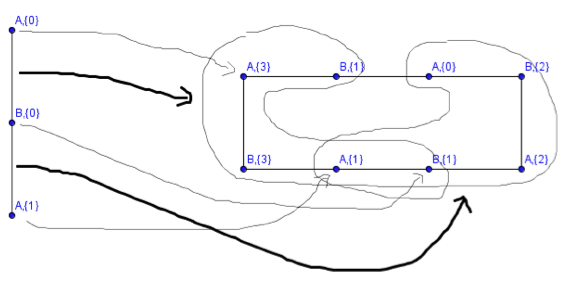
\includegraphics[scale=0.65]{Figura1.png}
    %%\end{center}

    \begin{enumerate}
      \item{Para los 2 modelos dados describe el complejo del protocólo para M. 
        Tienes que dar la tripleta $(I,P_m,\Xi_m)$}

      \item{Para los 2 modelos describe cuál es la tarea $\epsilon$-agreement
        óptima para cada \textit{M} $≥$ 0. Nos referimos a óptimo como que cada
        vista del protocolo va a un valor de decisión único. En otras palabras
      encontrar la $\epsilon$ en función de M.}
    \end{enumerate}
  }

\item{
    Con el modelo visto en clase define la función de decisión de equidad de género
    $\delta$, que no distingue entre Alice y Bob. Es decir Alice y Bob pueden tener
    ya sea el valor 0 o 1 de entrada. También da la $\delta$ óptima para este caso.
    Aqui debes de tener cuidado de como etiquetas los vértices para que siempre
    se cumpla la $\epsilon$.
  }

\item{
    
    Ahora regresamos al modelo de memoria compartida y modifiquémoslo. Ahora 
    supongamos que tenemos solo una memoria. Es decir ya no tenemos capas y
    sobreescribimos nuestra parte del arreglo cada ronda. También regresamos
    al caso en que Alice propone 0 y Bob 1.
    \begin{enumerate}
      
    \item{Describe el modelo (haz la gráfica) y ve como se ve la gráfica de 
        vistas después de M rondas.
      }

    \item{¿Cuál es la mejor $\epsilon$ que puede resolver en la tarea del 
        $\epsilon$-agreement en M rondas?}
    \end{enumerate}
  }

\end{enumerate}
\end{document}